
\begin{abox}
	Problem Set -1
\end{abox}
\begin{enumerate}[label=\color{ocre}\textbf{\arabic*.}]
	\item  Let $p_{n}(x)$ (where $n=0,1,2, \ldots \ldots$ ) be a polynomial of degree $n$ with real coefficients, defined in the interval $2 \leq n \leq 4$. If $\int_{2}^{4} p_{n}(x) p_{m}(x) d x=\delta_{n m}$, then
	{\exyear{NET/JRF(JUNE-2011)}}
	\begin{tasks}(2)
		\task[\textbf{A.}] $p_{0}(x)=\frac{1}{\sqrt{2}}$ and $p_{1}(x)=\sqrt{\frac{3}{2}}(-3-x)$
		\task[\textbf{B.}]  $p_{0}(x)=\frac{1}{\sqrt{2}}$ and $p_{1}(x)=\sqrt{3}(3+x)$
		\task[\textbf{C.}] $p_{0}(x)=\frac{1}{2}$ and $p_{1}(x)=\sqrt{\frac{3}{2}}(3-x)$
		\task[\textbf{D.}] $p_{0}(x)=\frac{1}{\sqrt{2}}$ and $p_{1}(x)=\sqrt{\frac{3}{2}}(3-x)$
	\end{tasks}
	\begin{answer}
		$$\int_{2}^{4} p_{n}(x) p_{m}(x) d x=\delta_{n m}$$
		For $n\neq m$,  $\delta_{n m}=0$. \\ One positive and one negative term can make integral zero. So answer may be (C) or (D). Now take $n=m=0$ so $p_{0}(x)=\frac{1}{\sqrt{2}}$ and then integrate. (D) is correct option because it satisfies the equation Check by integration and by orthogonal property of Legendre polynomial also.\\\\
		So the correct answer is \textbf{Option (D)}
	\end{answer}
	\item  The generating function $F(x, t)=\sum_{n=0}^{\infty} P_{n}(x) t^{n}$ for the Legendre polynomials $P_{n}(x)$ is $F(x, t)=\left(1-2 x t+t^{2}\right)^{-1 / 2}$. The value of $P_{3}(-1)$ is
	{\exyear{NET/JRF(DEC-2011)}}
	\begin{tasks}(4)
		\task[\textbf{A.}] $5 / 2$
		\task[\textbf{B.}] $3 / 2$
		\task[\textbf{C.}] $+1$
		\task[\textbf{D.}] $-1$
	\end{tasks}
	\begin{answer}
		\begin{align*}
		P_{3}&=\frac{1}{2}\left(5 x^{3}-3 x\right) \Rightarrow P_{3}(-1)\\&=\frac{1}{2}\left(5(-1)^{3}-3(-1)\right)=\frac{1}{2}[-5+3]=-1
		\end{align*}
		So the correct answer is \textbf{Option (D)}
	\end{answer}
	\item  The graph of the function $f(x)$ shown below is best described by
	{\exyear{NET/JRF(DEC-2012)}}
	\begin{figure}[H]
		\centering
		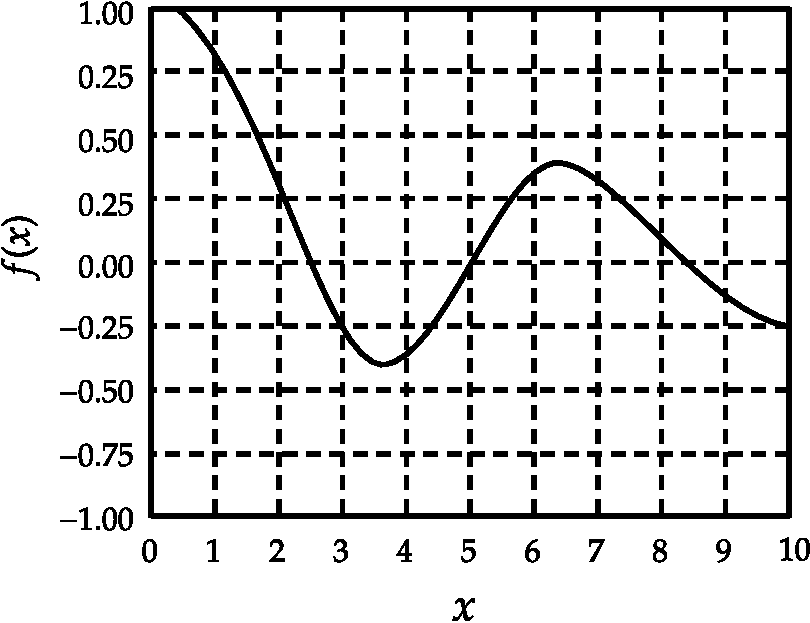
\includegraphics[height=6cm,width=8cm]{diagram-20211005(12)-crop}
	\end{figure}
	\begin{tasks}(2)
		\task[\textbf{A.}]  The Bessel function $J_{0}(x)$
		\task[\textbf{B.}] $\cos x$
		\task[\textbf{C.}] $e^{-x} \cos x$
		\task[\textbf{D.}] $\frac{1}{x} \cos x$
	\end{tasks}
	\begin{answer}
		So the correct answer is \textbf{Option (A)}
	\end{answer}
	\item Given that $\sum_{n=0}^{\infty} H_{n}(x) \frac{t^{n}}{n !}=e^{-t^{2}+2 t x}$ the value of $H_{4}(0)$ is
	{\exyear{NET/JRF(JUNE-2013)}}
	\begin{tasks}(4)
		\task[\textbf{A.}] 12
		\task[\textbf{B.}] 6
		\task[\textbf{C.}] 24
		\task[\textbf{D.}] $-6$
	\end{tasks}
	\begin{answer}
		\begin{align*}
		\sum_{n=0}^{\infty} H_{n}(x) \frac{t^{n}}{n !}&=e^{-t^{2}+2 x} \Rightarrow \sum_{n=0}^{\infty} H_{n}(0) \frac{t^{n}}{n !}\\&=e^{-t^{2}}=1-t^{2}+\frac{t^{4}}{2 !}-\frac{t^{6}}{3 !}\\
		\Rightarrow \frac{H_{4}(0)}{4 !} t^{4}&=\frac{t^{4}}{2 !} \Rightarrow H_{4}(0)=\frac{4 !}{2 !}=12
		\end{align*}
		So the correct answer is \textbf{Option (A)}
	\end{answer}
	\item   Given $\sum_{n=0}^{\infty} P_{n}(x) t^{n}=\left(1-2 x t+t^{2}\right)^{-1 / 2}$, for $|t|<1$, the value of $P_{5}(-1)$ is
	{\exyear{NET/JRF(JUNE-2014)}}
	\begin{tasks}(4)
		\task[\textbf{A.}] $0.26$
		\task[\textbf{B.}] 1
		\task[\textbf{C.}] $0.5$
		\task[\textbf{D.}] $-1$
	\end{tasks}
	\begin{answer}
		\begin{align*}
		P_{n}(-1)&=-1\text{ if }n\text{ is odd }\Rightarrow P_{5}(-1)=-1
		\end{align*}
		So the correct answer is \textbf{Option (D)}
	\end{answer}
	\item The function $f(x)=\sum_{n=0}^{\infty} \frac{(-1)^{n}}{n !(n+1) !}\left(\frac{x}{2}\right)^{2 n+1}$, satisfies the differential equation
	{\exyear{NET/JRF(DEC-2014)}}
	\begin{tasks}(2)
		\task[\textbf{A.}]  $x^{2} \frac{d^{2} f}{d x^{2}}+x \frac{d f}{d x}+\left(x^{2}+1\right) f=0$
		\task[\textbf{B.}]  $x^{2} \frac{d^{2} f}{d x^{2}}+2 x \frac{d f}{d x}+\left(x^{2}-1\right) f=0$
		\task[\textbf{C.}] $x^{2} \frac{d^{2} f}{d x^{2}}+x \frac{d f}{d x}+\left(x^{2}-1\right) f=0$
		\task[\textbf{D.}] $x^{2} \frac{d^{2} f}{d x^{2}}-x \frac{d f}{d x}+\left(x^{2}-1\right) f=0$
	\end{tasks}
	\begin{answer}
		\begin{align*}
		\intertext{ $f(x)=\sum_{n=0}^{\infty} \frac{(-1)^{n}}{n !(n+1) !}\left(\frac{x}{2}\right)^{2 n+1}$ is generating function (Bessel Function of first kind) which satisfies the differential equation $x^{2} \frac{d^{2} f}{d x^{2}}+x \frac{d f}{d x}+\left(x^{2}-n^{2}\right) f=0$, put $n=1$.}
		\end{align*}
		So the correct answer is \textbf{Option (C)}
	\end{answer}
	\item
	The Hermite polynomial $H_{n}(x)$, satisfies the differential equation
	$$
	\frac{d^{2} H_{n}}{d x^{2}}-2 x \frac{d H_{n}}{d x}+2 n H_{n}(x)=0
	$$
	The corresponding generating function $G(t, x)=\sum_{n=0}^{\infty} \frac{1}{n !} H_{n}(x) t^{n}$, satisfies the equation
	{\exyear{NET/JRF(DEC-2015)}}
	\begin{tasks}(2)
		\task[\textbf{A.}] $\frac{\partial^{2} G}{\partial x^{2}}-2 x \frac{\partial G}{\partial x}+2 t \frac{\partial G}{\partial t}=0$
		\task[\textbf{B.}] $\frac{\partial^{2} G}{\partial x^{2}}-2 x \frac{\partial G}{\partial x}-2 t^{2} \frac{\partial G}{\partial t}=0$
		\task[\textbf{C.}] $\frac{\partial^{2} G}{\partial x^{2}}-2 x \frac{\partial G}{\partial x}+2 \frac{\partial G}{\partial t}=0$
		\task[\textbf{D.}]  $\frac{\partial^{2} G}{\partial x^{2}}-2 x \frac{\partial G}{\partial x}+2 \frac{\partial^{2} G}{\partial x \partial t}=0$
	\end{tasks}
	\begin{answer}
		\begin{align*}
		G&=\frac{1}{n !} H_{n}(x) t^{n}, G^{\prime}=\frac{1}{n !} H_{n}^{\prime}(x) t^{n}, G^{\prime \prime}=\frac{1}{n !} H_{n}^{\prime \prime}(x) t^{n}\\
		\frac{\partial G}{\partial t}&=\frac{1}{n !} H_{n}(x) n t^{n-1}
		\intertext{Let's check the options one by one}
		\frac{\partial G}{\partial x^{2}}&-2 x \frac{\partial G}{\partial x}+2 t \frac{\partial G}{\partial t}=0\\
		\frac{1}{n !} H_{n}^{\prime \prime}(x) t^{n}&-2 x \frac{1}{n !} H_{n}^{\prime}(x) t^{n}+2 t \frac{1}{n !} H_{n}(x) n t^{n-1}\\
		H_{n}^{\prime \prime}(x)-2 x H_{n}^{\prime}(x)+2 x H_{n}(x)&=0,\text{ which is Hermite Differential Equation.}
		\end{align*}
		So the correct answer is \textbf{Option (A)}
	\end{answer}
	\item A stable asymptotic solution of the equation $x_{n+1}=1+\frac{3}{1+x_{n}}$ is $x=2$. If we take $x_{n}=2+\epsilon_{n}$ and $x_{n+1}=2+\epsilon_{n+1}$, where $\epsilon_{n}$ and $\epsilon_{n+1}$ are both small, the ratio $\frac{\epsilon_{n+1}}{\epsilon_{n}}$ is approximately
	{\exyear{NET/JRF(DEC-2016)}}
	\begin{tasks}(4)
		\task[\textbf{A.}] $-\frac{1}{2}$
		\task[\textbf{B.}] $-\frac{1}{4}$
		\task[\textbf{C.}]  $-\frac{1}{3}$
		\task[\textbf{D.}] $-\frac{2}{3}$
	\end{tasks}
	\begin{answer}
		So the correct answer is \textbf{Option (C)}
	\end{answer}
	
	\item  The generating function $G(t, x)$ for the Legendre polynomials $P_{n}(t)$ is
	$$
	G(t, x)=\frac{1}{\sqrt{1-2 x t+x^{2}}}=\sum_{n=0}^{\infty} x^{n} P_{n}(t), \text { for }|x|<1
	$$
	If the function $f(x)$ is defined by the integral equation $\int_{0}^{x} f\left(x^{\prime}\right) d x^{\prime}=x G(1, x)$, it can be expressed as
	{\exyear{NET/JRF(DEC-2017)}}
	\begin{tasks}(2)
		\task[\textbf{A.}] $\sum_{n, m=0}^{\infty} x^{n+m} P_{n}(1) P_{m}\left(\frac{1}{2}\right)$
		\task[\textbf{B.}] $\sum_{n, m=0}^{\infty} x^{n+m} P_{n}(1) P_{m}(1)$
		\task[\textbf{C.}] $\sum_{n, m=0}^{\infty} x^{n-m} P_{n}(1) P_{m}(1)$
		\task[\textbf{D.}] $\sum_{n, m=0}^{\infty} x^{n-m} P_{n}(0) P_{m}(1)$
	\end{tasks}
	\begin{answer}
		\begin{align*}
		G(t, x)&=\frac{1}{\sqrt{1-2 x t+x^{2}}}=\sum_{n=0}^{\infty} x^{n} P_{n}(t)\text{ for }|x|<1\\
		G(1, x)&=\frac{1}{\sqrt{1-2 x+x^{2}}}=\sum_{n=0}^{\infty} x^{n} P_{n}(1)\\
		\sum_{n=0}^{\infty} x^{n} P_{n}(1)&=\frac{1}{\sqrt{(1-x)^{2}}}\\&=\frac{1}{1-x}\text{ Since } |x|<1\\
		\text{Now, }x \cdot \frac{1}{1-x}&=\int_{0}^{x} f\left(x^{\prime}\right) d x^{\prime}
		\intertext{Differentiating both sides,}
		f(x)&=\frac{d}{d x} \frac{x}{1-x}=\frac{1}{(1-x)^{2}}
		\intertext{Which can be represented as,}
		\sum_{n, m=0}^{\infty} x^{n+m} P_{n}(1) P_{m}(1)&=\frac{1}{(1-x)^{2}}
		\end{align*}
		So the correct answer is \textbf{Option (B)}
	\end{answer}
	\item In the function $P_{n}(x) e^{-x^{2}}$ of a real variable $x, P_{n}(x)$ is polynomial of degree $n$. The maximum number of extrema that this function can have is
	{\exyear{NET/JRF(JUNE-2018)}}
	\begin{tasks}(4)
		\task[\textbf{A.}] $n+2$
		\task[\textbf{B.}]  $n-1$
		\task[\textbf{C.}] $n+1$
		\task[\textbf{D.}] $n$
	\end{tasks}
	\begin{answer}
		\begin{align*}
		y&=P_{n}(x) e^{-x^{2}} \Rightarrow P_{n}^{\prime}(x) e^{-x^{2}}+P_{n}(x) e^{-x^{2}}(-2 x)\\
		&=0 \Rightarrow P_{n}^{\prime}(x)-2 x P_{n}(x)=0\\
		P_{0}(x)=1, P_{1}(x)&=2 \Rightarrow P_{0}^{\prime}(x)-2 x P_{0}(x)\\&=0 \Rightarrow 0-2 x .1=0\\
		x&=0,1\text{ extrema}\\
		P_{1}^{\prime}(x)-2 x P_{1}(x)&=0\\
		1-2 x \cdot x&=0 \Rightarrow x=\pm \frac{1}{\sqrt{2}}\text{ i.e., 2 extrema.}\\
		\text{Thus in general there are }&(n+1)\text{ extrema.}
		\end{align*}
		So the correct answer is \textbf{Option (C)}
	\end{answer}
	
	\item The polynomial $f(x)=1+5 x+3 x^{2}$ is written as linear combination of the Legendre polynomials
	$\left(P_{0}(x)=1, P_{1}(x), P_{2}(x)=\frac{1}{2}\left(3 x^{2}-1\right)\right)$ as $f(x)=\sum_{n} c_{n} P_{n}(x)$. The value of $c_{0}$ is
	{\exyear{NET/JRF(DEC-2018)}}
	\begin{tasks}(4)
		\task[\textbf{A.}] $\frac{1}{4}$
		\task[\textbf{B.}] $\frac{1}{2}$
		\task[\textbf{C.}]  2
		\task[\textbf{D.}]  4
	\end{tasks}
	\begin{answer}
		\begin{align*}
		f(x)&=1+5 x+3 x^{2}\\
		1&=P_{0}(x) \quad x=P_{1}(x)\\
		x^{2}&=\frac{1}{3}\left(2 P_{2}(x)+1\right)\\
		f(x)&=P_{0}(x)+5 P_{1}(x)+2 P_{2}(x)+P_{0}(x)\\
		&=2 P_{0}(x)+5 P_{1}(x)+2 P_{2}(x)\\
		&=c_{0} P_{0}(x)+c_{1} P_{1}(x)+c_{2} P_{2}(x) c_{0}=2
		\end{align*}
		So the correct answer is \textbf{Option (C)}
	\end{answer}
	
	
\end{enumerate}
\colorlet{ocre1}{ocre!70!}
\colorlet{ocrel}{ocre!30!}
\setlength\arrayrulewidth{1pt}
\begin{table}[H]
	\centering
	\arrayrulecolor{ocre}
	\begin{tabular}{|p{1.5cm}|p{1.5cm}||p{1.5cm}|p{1.5cm}|}
		\hline
		\multicolumn{4}{|c|}{\textbf{Answer key}}\\\hline\hline
		\rowcolor{ocrel}Q.No.&Answer&Q.No.&Answer\\\hline
		1&\textbf{D} &2&\textbf{D}\\\hline 
		3&\textbf{A} &4&\textbf{A} \\\hline
		5&\textbf{D} &6&\textbf{C} \\\hline
		7&\textbf{A}&8&\textbf{C}\\\hline
		9&\textbf{B}&10&\textbf{C}\\\hline
		11&\textbf{C} &&\\\hline
		
		
	\end{tabular}
\end{table}
\begin{abox}
	Problem Set -3
\end{abox}
\begin{questions}
\begin{minipage}{\textwidth}
	\question What is the maximum number of extrema of the function $f(x)=P_{k}(x) e^{-\left(\frac{x^{4}}{4}+\frac{x^{2}}{2}\right)}$, where\\
	$x \in(-\infty, \infty)$ and $P_{k}(x)$ is an arbitrary polynomial of degree $k$ ?
	\exyear{JEST 2015}
\end{minipage}
\begin{tasks}(4)
	\task[\textbf{A.}]  $k+2$
	\task[\textbf{B.}]$k+6$
	\task[\textbf{C.}] $k+3$
	\task[\textbf{D.}]$k$
\end{tasks}
\begin{answer}
	\begin{align*}
	f(x)&=P_{x}(x) e^{-\left(\frac{x^{4}}{4}+\frac{x^{2}}{2}\right)}\\
	f^{\prime}(x)&=\left[P_{x}^{\prime}(x)+P_{x}(x)(-1)\left(x^{3}+x\right)\right] e^{-\left(\frac{x^{4}}{4}+\frac{x^{2}}{2}\right)}\\
	\intertext{For maximum number of extrema,}
	\Rightarrow f^{\prime}(x)&=0 \Rightarrow\left[P_{x}(x)\left(x^{3}+x\right)-P^{\prime}(x)\right]=0 \intertext{ Then it is a polynomial of order  $ k+3 $}
	\intertext{From the sign scheme maximum number of extrema $ =k+3 $ }
	\end{align*}
	Correct option is (C)
\end{answer}
\begin{minipage}{\textwidth}
	\question The Bernoulli polynominals $B_{n}(s)$ are defined by, $\frac{x e^{x s}}{e^{x}-1}=\sum B_{n}(s) \frac{x^{n}}{n !} .$ Which one of the following relations is true?
	\exyear{JEST 2015}
\end{minipage}
\begin{tasks}(2)
	\task[\textbf{A.}] $\frac{x e^{x(1-s)}}{e^{x}-1}=\sum B_{n}(s) \frac{x^{n}}{(n+1) !}$
	\task[\textbf{B.}]$\frac{x e^{x(1-s)}}{e^{x}-1}=\sum B_{n}(s)(-1)^{n} \frac{x^{n}}{(n+1) !}$
	\task[\textbf{C.}]$\frac{x e^{x(1-s)}}{e^{x}-1}=\sum B_{n}(-s)(-1)^{n} \frac{x^{n}}{n !}$
	\task[\textbf{D.}]$\frac{x e^{x(1-s)}}{e^{x}-1}=\sum B_{n}(s)(-1)^{n} \frac{x^{n}}{n !}$
\end{tasks}
\begin{answer}
	\begin{align*}
	\frac{x e^{x s}}{e^{x}-1}&=\sum B_{n}(s) \frac{x^{n}}{ n!}
	\intertext{Put  $ s=(s-1),$ Then,}   \frac{x e^{x(s-1)}}{e^{x}-1}&=\sum B_{n}(s-1) \frac{x^{n}}{ n!}\\
	\text{Since, }\ B_{n}(s-1)&=(-1)^{n} B(s)\\
	\Rightarrow \frac{x e^{x(s-1)}}{e^{x}-1}&=\sum B_{n}(s)(-1)^{n} \frac{x^{n}}{ n!}
	\end{align*}
	Correct option is (D)
\end{answer}



\begin{minipage}{\textwidth}
	\question For which of the following conditions does the integral $\int_{0}^{1} P_{m}(x) P_{n}(x) d x$ vanish for $m \neq n$, where $P_{m}(x)$ and $P_{n}(x)$ are the Legendre polynomials of order $m$ and $n$ respectively?
	\exyear{JEST 2018}
\end{minipage}
\begin{tasks}(2)
	\task[\textbf{A.}] all $m, m \neq n$
	\task[\textbf{B.}]$m-n$ is an odd integer
	\task[\textbf{C.}]$m-n$ is a nonzero even integer
	\task[\textbf{D.}]$n=m \pm 1$
\end{tasks}
\begin{answer}
	\begin{align*}
	\int_{-1}^{1} P_{m}(x) P_{n}(x) d x&=\frac{2}{2 x+1} \delta_{n m}\\
	2 \int_{0}^{1} P_{m}(x) P_{n}(x) d x&=\frac{2}{2 x+1} \delta_{n m}\\
	\text{Only } P_{m}(x) P_{n}(x)&= \text{even}\\
	&m\\
	&0 \quad \text{even}\\
	&1 \quad \text{odd}\\
	&2 \quad \text{even}\\
	&3 \quad \text{odd}\\
	&4 \quad \text{even}\\
	m-n&= \text{non zero even integer then only}\\
	P_{m}(x) P_{n}(x)&= \text{even}\\
	m \neq n \ \Delta \delta_{n m}&=0
	\end{align*}
	Correct option is (A)
\end{answer}
\begin{minipage}{\textwidth}
	\question The Euler polynomials are defined by $\frac{2 e^{x s}}{e^{x}+1}=\sum_{n=0}^{\infty} E_{n}(s) \frac{x^{n}}{n !}$What is the value of $E_{5}(2)+E_{5}(3) ?$
	\exyear{JEST 2019}
\end{minipage}
\begin{answer}
	\begin{align*}
	\frac{2 e^{x s}}{e^{x}+1}=&\sum_{n=0}^{\infty} E_{n}(s) \frac{x^{n}}{n !}\\
	E_{n}(x+1)+E_{n}(x)&=2 x^{n}\\
	E_{5}(x+1)+E_{5}(x)&=2 x^{5}\\
	c&=2=2 \times 2^{5}\\&=64\\
	\end{align*}
\end{answer}

\begin{minipage}{\textwidth}
	\question If $F(x, y)=x^{2}+y^{2}+x y$, its Legendre transformed function $G(u, v)$, upto a multiplicative constant, is
	\exyear{JEST 2018}
\end{minipage}
\begin{tasks}(4)
	\task[\textbf{A.}] $u^{2}+v^{2}+u v$
	\task[\textbf{B.}] $u^{2}+v^{2}-u v$
	\task[\textbf{C.}]$u^{2}+v^{2}$
	\task[\textbf{D.}]$(u+v)^{2}$
\end{tasks}
\begin{answer}
	\begin{align*}
	G&=F-x u-y v\\
	d G&=d F-x d u-u d v-y d v-v d y\\
	F&=x^{2}+y^{2}+x y\\
	d F&=\frac{\partial F}{\partial x} d x+\frac{\partial F}{\partial y} d y\\
	d F&=u d x+v d y\\
	d G&=u d x+v d y-x d u-u d x-y d v-v d y\\
	d G&=-x d u-y d v\\
	u&=\frac{\partial F}{\partial x}, v=\frac{\partial F}{\partial x}\\
	u&=2 x+y, 2 u=4 x+2 y\\
	2 v&=4 y+2 x, v=2 y+x\\
	y&=+\frac{1}{3}[2 v-u]\\
	2 u-v&=3 x\\
	x&=\frac{1}{3}[2 u-v]\\
	d G&=-\frac{1}{3}[2 u-v] d u-\frac{1}{3}[2 v-u] d x\\
	d G(u, v)&=-\frac{1}{3}(2 u-v) d u-\frac{1}{3}(2 v-u) d v=\frac{\partial G}{\partial u} d u+\frac{\partial G}{\partial v} d v\\
	\frac{\partial G}{\partial u}&=-\frac{1}{3}(2 u-v), \frac{\partial G}{\partial v}=-\frac{1}{3}(2 v-u)\\
	G(u, v)&=-\frac{1}{3}\left(u^{2}-u v\right)+h(v)\\
	G(u, v)&=-\frac{1}{3}(-u)+\frac{d h(v)}{d(v)}=\frac{u}{3}+\frac{d h(v)}{d v}\\
	\frac{-2 v}{3}+\frac{u}{3}&=\frac{u}{3}+\frac{d h(v)}{d x}\\
	h(v)&=\frac{-v^{2}}{3}\\
	G(u, v)&=-\frac{1}{3}\left(u^{2}-u v\right)-\frac{v^{2}}{3}=-\frac{1}{3}\left(u^{2}+v^{2}-u v\right)
	\end{align*}
	Correct option is (B)
\end{answer}
\begin{minipage}{\textwidth}
	\question Consider a function $f(x)=P_{k}(x) e^{-\left(x^{4}+2 x^{2}\right)}$ in the domain $x \in(-\infty, \infty)$, where $P_{k}$ is any polynomial of degree $k$. What is the maximum possible number of extrema of the function?
	\exyear{JEST 2019}
\end{minipage}
\begin{tasks}(4)
	\task[\textbf{A.}] $k+3$
	\task[\textbf{B.}] $k-3$
	\task[\textbf{C.}]$k+2$
	\task[\textbf{D.}]$k+1$
\end{tasks}
\begin{answer}
	\begin{align*}
	f(x)&=p_{k}(x) e^{-\left(x^{4}+2 x^{2}\right)}\\
	\text{Let } k=0, f(x)&=p_{0}(x) e^{-\left(x^{4}+2 x^{2}\right)}\\
	\text{Number of extrema}\\
	P_{0}(x)&=1, k=0\\
	\text{Number of extrema} &=1\\
	k+1&=0+1=1
	\end{align*}
	\begin{figure}[H]
		\begin{center}
			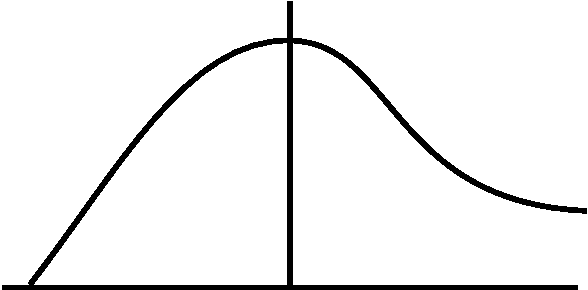
\includegraphics[width=3.5cm,height=2.5cm]{59-S-crop}
		\end{center}
	\end{figure}
\end{answer}
\end{questions}
\colorlet{ocre1}{ocre!70!}
\colorlet{ocrel}{ocre!30!}
\setlength\arrayrulewidth{1pt}
\begin{table}[H]
	\centering
	\arrayrulecolor{ocre}
	\begin{tabular}{|p{1.5cm}|p{1.5cm}||p{1.5cm}|p{1.5cm}|}
		\hline
		\multicolumn{4}{|c|}{\textbf{Answer key}}\\\hline\hline
		\rowcolor{ocrel}Q.No.&Answer&Q.No.&Answer\\\hline
		1&\textbf{C} &2&\textbf{D}\\\hline 
		3&\textbf{A} &4&\textbf{64} \\\hline
		5&\textbf{B} &6&\textbf{D} \\\hline
		
		
	\end{tabular}
\end{table}